
\begin{figure*}[thbp!]
\centering
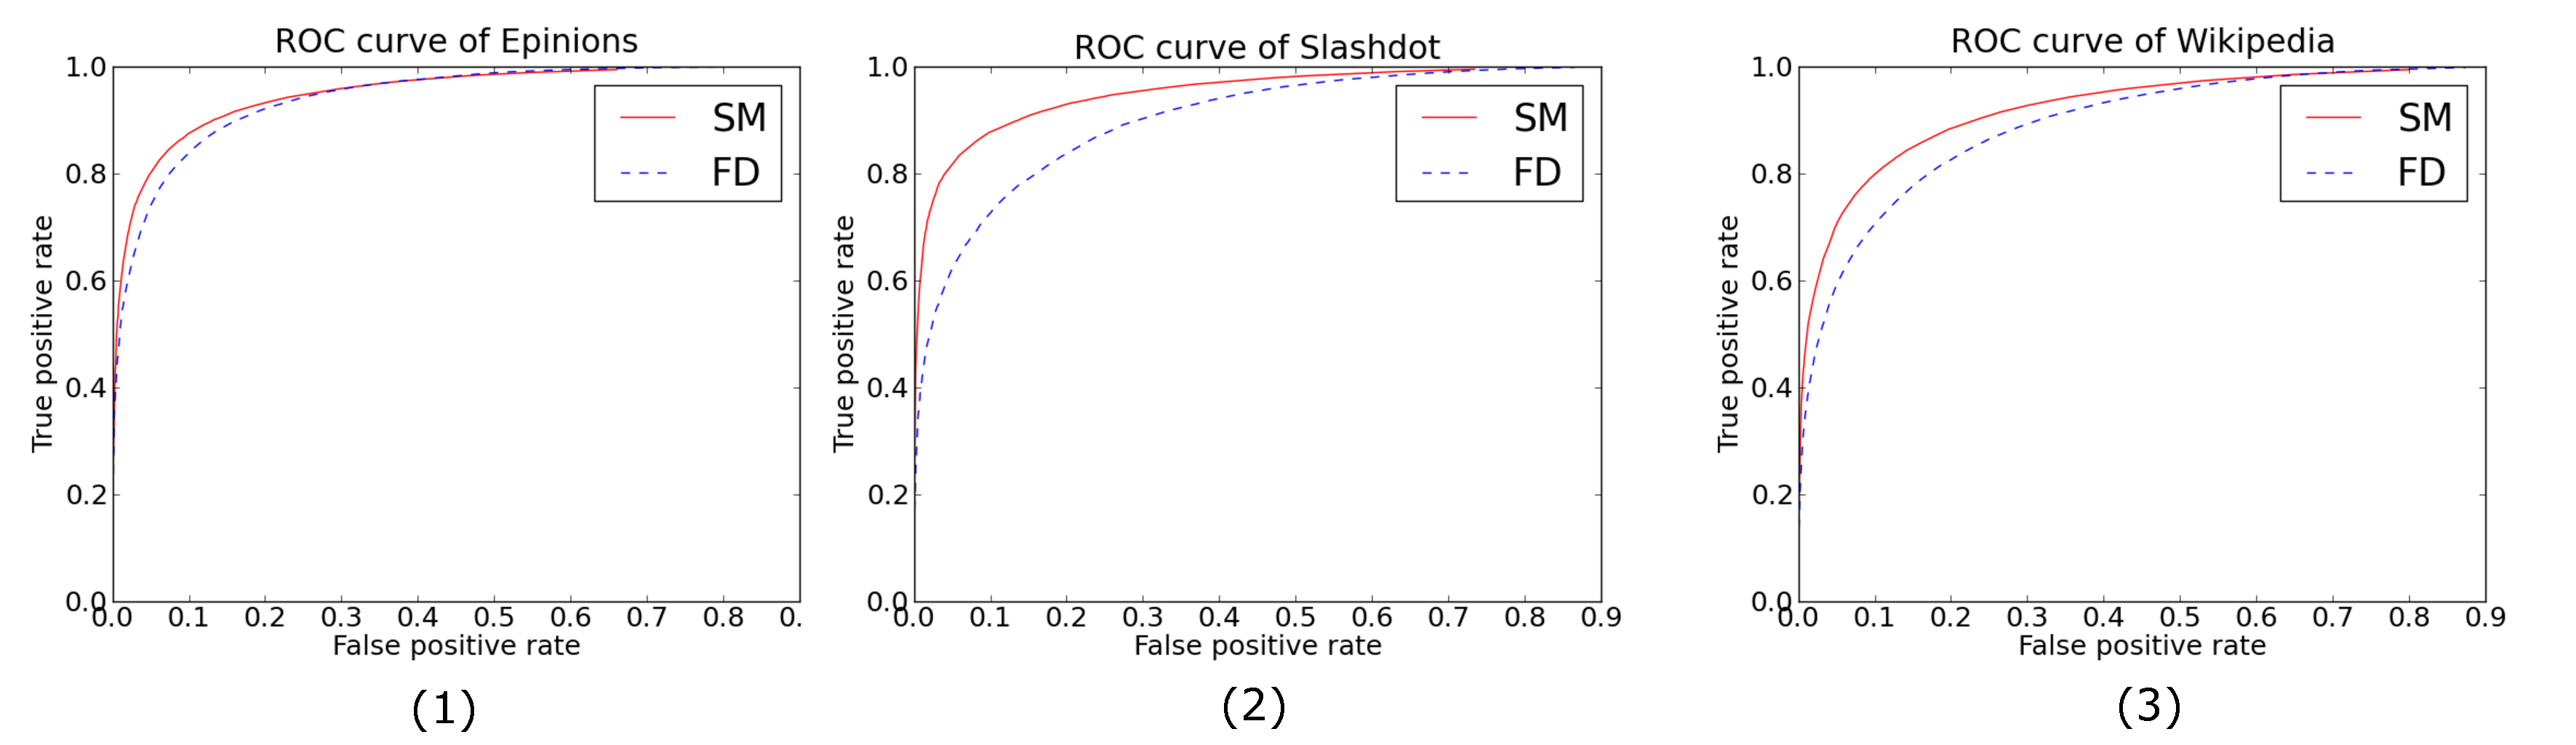
\includegraphics[height=2in]{Figs/ROC_curve_hor.pdf}
\vspace*{-0.1in}
\caption{\label{fig:ROC} The ROC curves are drawn upon distances of
  hidden edges, generated by SM and FD for (1) Epinions, (2) Slashdot
  and (3) Wikipedia datasets.}
\end{figure*}


\section{Experimental Results} \label{sec:results}
In this section, we first focus on the {\it edge sign prediction
  problem}. Suppose we are given a social network with signs, but a
small fraction of the edge signs are ``hidden''. How can we predict
these signs with the information provided by the rest of network?
The convergence model is able to predict these ``hidden'' signs. Let's
denote the original social network with all signed edges as $G$, the
network consisting of hidden edges as $G_{h}$, and the network
consisting of the remaining edges as $G_{r}$. The edges (relations)
between each pair of nodes is measured by $\{+,\,-,\,O\}$. We run the
convergence model on $G_{r}$, and denote the network after convergence
as $G_{r}^{'}$. We expect that the signs of the hidden edges in
$G_{r}^{'}$ largely agree with the true signs.

By the assumption that every social network has a tendency towards
balance, it can be inferred that $G$ is largely balanced at any
moment. Hence, the majority of $G_{r}$ is balanced. The only
exceptions are the components with hidden edges, which are of sign $O$
in $G_{r}$. By the principle of total relation cost minimization, the
changes mostly occur on the $O$-sign hidden edges during the
convergence. We expect the hidden edges in $G_h$ to have their
true signs in $G_{r}^{'}$ if $G$ is largely balanced.

We compare our algorithm to force directed algorithm (FD)
in~\cite{golbeck:distrust2011}. Note that we have tuned our
implementation of FD to provide similar performance reported in this
work. Even though this work combines two algorithms, in our comparison
experiments, we find that FD alone gives equally good prediction
performance on all three datasets as the combination. Due to space
limitations, we exclude the detailed study of PP and FD/PP combination
from this paper.


\begin{algorithm}~\label{alg}
 \KwData{$M, k, deg, G$}
 \KwResult{$Pt, Nt$}
 Get $G'=$ generate-subgraph$(M, k, deg, G)$\;
 Partition $G'$ into 10 groups of test and training samples\;
 Create two empty sets $Pt$, $Nt$\;
 \For{each of the groups}{
 run SM on the training sample and get the layout\;
 \For{each edge e in the testing sample}{
 compute its distance in the layout\;
 \eIf{e is a positive edge}{
   add its distance to $Pt$\;
   }{
   add its distance to $Nt$\;
  }
 }
 }
 \caption{SM Prediction}
\end{algorithm}

We use the same three datasets as it is
in~\cite{golbeck:distrust2011}~\cite{Leskovec:2010} to conduct our
experiments, all provided by the Stanford Large Network Dataset
Collection. (1) {\em Epinions} is a product review website where users
give reviews and ratings on product articles. Users can choose to
trust or distrust others. The network contains more than 100,000 users
and over 700,000 trust/distrust edges. (2) {\em Slashdot} is a
technology news website where users rate each other as friends or
foes. The dataset released in February 2009 contains over 77,000 users
and over 900,000 friend/foe edges. (3) {\em Wikipedia} elections
collects the votes by Wikipedia users in elections for promoting
candidates as administrators. Each user can give a supporting
(positive) or opposing (negative) vote on the promotion of
another. The dataset has about 7,000 users and around 100,000 votes
(edges).

All edges are treated as undirected. Running SM on the entire dataset
is infeasible due to both the memory and computational cost. As a
result, we generate random samples of our datasets using snowball
sampling method in which a small number $k$ of seeds with degree
greater than a given threshold $deg$ are selected at random, then all
nodes that are adjacent to the seed node are selected iteratively
until the desired network size is reached.  In our practice, the size
of the resulting graph is in the range 3,000-5,000 nodes, $k$ is
chosen from 2-10 randomly and $deg$ is chosen from 7-20 randomly. For
each dataset, we generate 10 sub-networks and perform 10-fold cross
validation. The number of edges in a sub-network of Epinions is around
180,000, for Slashdot 65,000 and for Wikipedia 160,000. In the
implementation of SM, the partitioning of the distance domain
satisfies $b_{+} < 1/2b_{-}$, conforming to our theory. The weight of
each type of edge satisfies $w_{O}<<w_{+}<1/2w_{-}$. The first
inequality has been argued in previous section. The second one is
chosen empirically, indicating that a negative edge has larger
influence than a positive one. We use the same setting for all the
networks and do not employ any other adjustable parameters.


\begin{figure*}[thbp!]
\centering
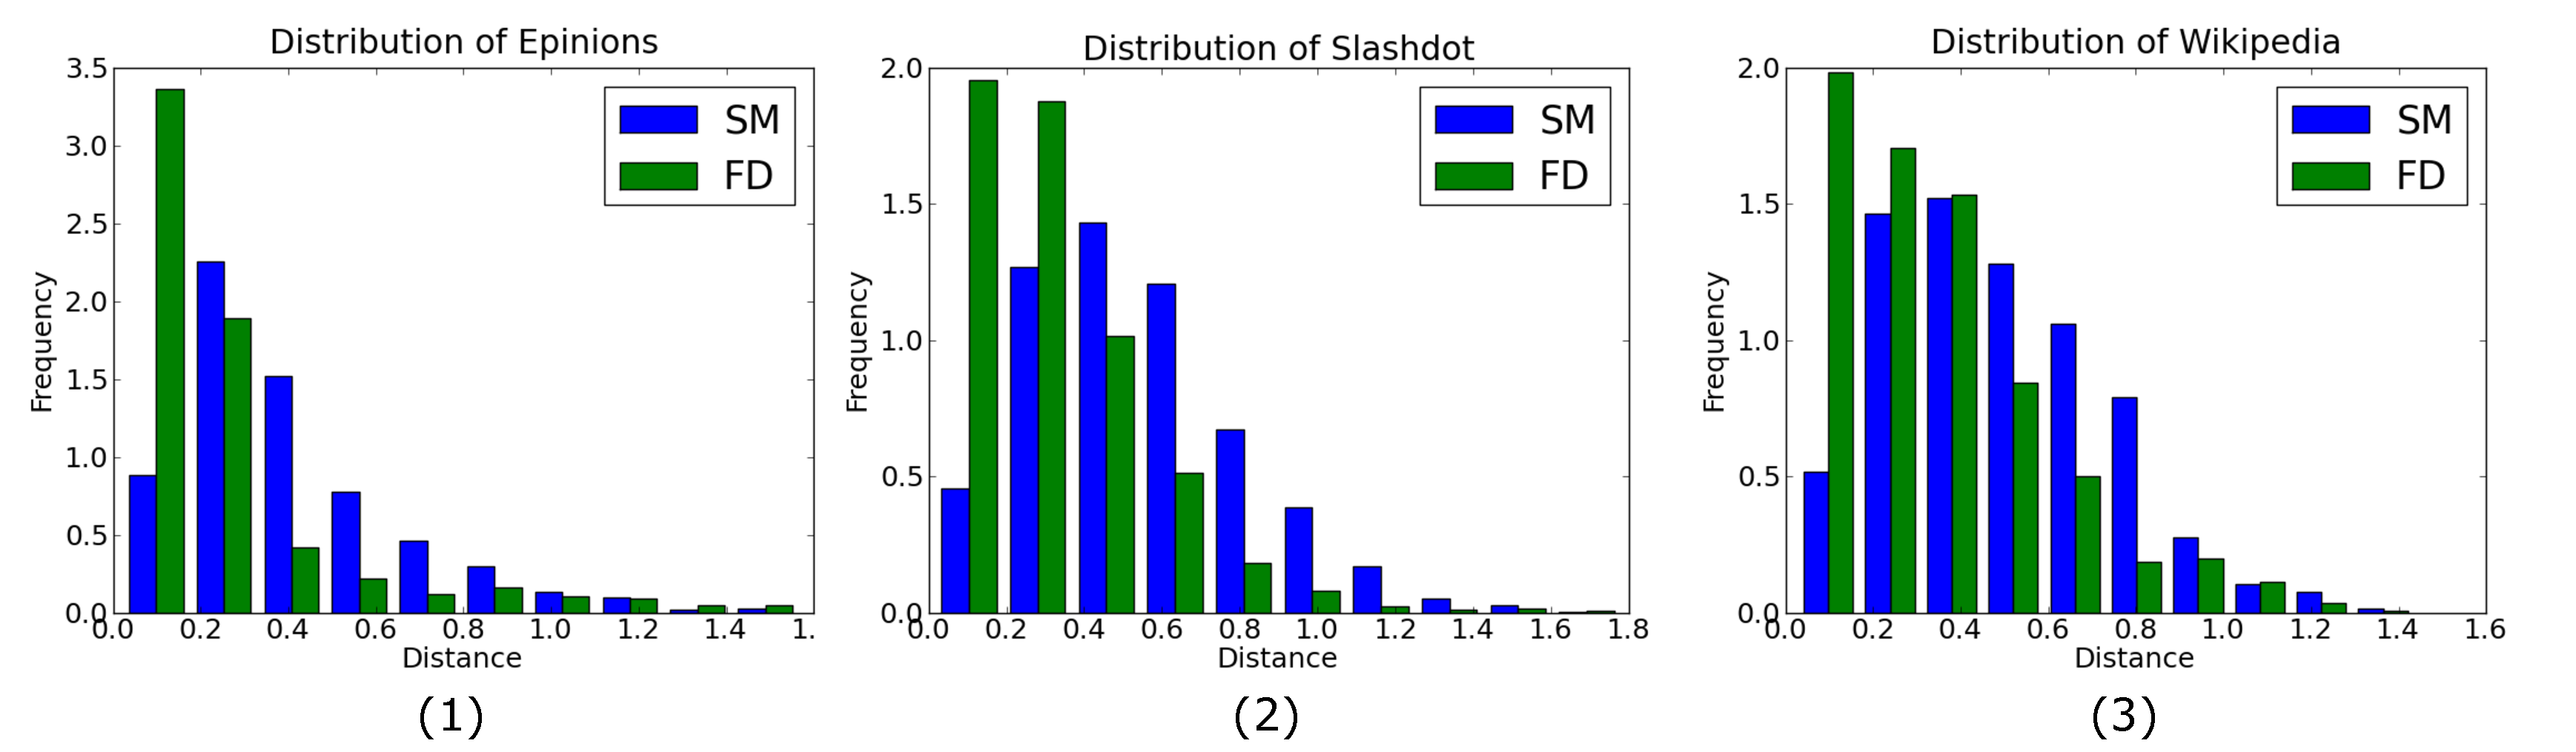
\includegraphics[height=2in]{Figs/hist1_hor.pdf}
\vspace*{-0.1in}
\caption{\label{hist} The histograms are drawn upon distances of
  neutral testing edges, generated by SM and FD for (1) Epinions, (2)
  Slashdot and (3) Wikipedia datasets.}
\end{figure*}

\noindent {\bf Edge Sign Prediction.} The distances of testing edges
are computed by the layout of the training data. Given a distance
threshold, the sign of each edge is predicted as positive if and only
if its distance is smaller than the threshold. In the previous work,
such threshold is computed from the (distance,sign) pairs of the
training samples using standard machine learning
techniques~\cite{golbeck:distrust2011}\cite{Leskovec:2010}. In this
paper, however, we do not concentrate on the learning process. The
issue of interest is how good the convergence model performs in
separating hidden positive edges from negative ones in terms of
distance. Instead of making predictions based on a particular
threshold, we draw ROC curves for evaluation which capture the
performance of sign prediction for both positive and negative edges
across all thresholds and compute the false and true positive rates
based on the computed $Pt$ ($Nt$) values returned by the
Algorithm~\ref{alg}. The ROC curves in Figure~\ref{fig:ROC} are drawn
upon the $Pt$ ($Nt$) values from the accumulation of all testing
samples.

For all three datasets, we find the ROC curve of $SM$ is on the
``northwest'' side of the one of $FD$, which indicates $SM$ is
consistently better than $FD$ in separating hidden positive edges from
negative ones. Notice that the improvement for Slashdot is the most
significant one among the three, possibly due to the fact that
Slashdot edges represent ``friends'' or ``foes'', which is by nature a
more clear identification of trust/distrust compared to votes in
Wikipedia or distrust for reviews in Epinions.  As a result, our
convergence model produces a very good prediction performance.  On the
Epinions and Slashdot datasets, the best thresholds on ROC curve give
$88-90 \%$ accuracy on both positive and negative hidden edges. For
Wikipedia, $SM$ achieves $83-85 \%$ at the best threshold. The
accuracy rates of Epinions and Wikipidea match the best results from
previous work, and Slashdot appears to be the best so far.

\noindent {\bf General Link Prediction.} The {\it edge sign
  prediction} only deals with the cases in which we already know that
an edge exists in the original network. A more general and harder
problem is to predict whether there is a positive edge between a pair of nodes (link prediction~\cite{Kleinberg:03}). The
difficulty of these problems stem from the fact that social networks
are usually sparse with a lot more neutral relations than biased
relations. Our convergence model should be able to make general edge
predictions based on distances. If larger distances represent more
negativeness (less positiveness), then the distance of a neutral
relation should be smaller than a negative one and larger than a
positive one. As a consequence, the distribution of neutral edges in
terms of distance should concentrate in the middle range. We study
this distribution, as a preliminary step towards solving the general
edge prediction.

For each dataset, we generate samples based on random source nodes as
before, except that we exclude the edges between the $k$ source
nodes. Instead of cross validation, we use the entire sub-network for
training, and use the $k(k-1)/2$ edges between the $k$ source nodes as
testing data, whose signs are available in the original dataset
(positive, negative or neutral, i.e. no link). %% Similarly, the signs of
%% the testing edges should not be influenced strongly by the other edges
%% in the network. Hence, a
After convergence the distances of these edges should be
representative of their true signs. We repeat the experiments 50 times
over all three datasets, and collect the distances for only the
neutral testing edges. Figure~\ref{hist} shows that the distances of
neutral testing edges generated by SM do relatively concentrate in the
middle-range of values following an almost Gaussian distribution. In
contrast, the majority of neutral testing edges's distances by FD have
small values, implying a positive prediction is much more likely for
FD than for SM.  However, SM provides more flexibility as the
distances are distributed over a larger range with an almost Gaussian
distribution, allowing us to test different tunable algorithms.
%% The experimental results show the superiority of our convergence model
%% in predicting signed edges. Moreover, they justify that our general
%% balance theory is a relatively accurate description of the stable
%% state of social networks, and that the convergence model correctly
%% characterizes the dynamics of social network.
As a result, our model
is a good starting point for developing algorithms for solving the general
{\it link prediction problem}.
